%Implementation, Integration and Test Plan

\subsection{Integration conditions}

\subsubsection{Entry Criteria}

Integration and testing processes should be performed on each single unit as soon as the component has been fully developed. In addition, integration of different components should be perform only if all these criteria are satisfied:

\begin{itemize}
	\item RASD and DD documents can be considered "stable", therefore it isn't expected any other modification of requirements or structure of the system, furthermore both deliverables ought to be distributed to all developer team involved in the project.
	\item There are same dependencies in integration and testing plan that have to be satisfied in order to guarantee the possibility to perform useful cross-components tests on functionalities, because of intrinsic bounds of the architecture.
	\begin{enumerate}
		\item \textit{Map Services} and \textit{Route Services} for \textit{RouteManager}
		\item \textit{SMS Gateway} and \textit{Push Gateway} for \textit{NotificationManager}
		\item \textit{Map Services} for \textit{MA} and \textit{WebUI}
		\item \textit{DBMS} for \textit{CalendarManager}, \textit{ReportManager} and \textit{PreferenceManager}
		\end{enumerate}
\end{itemize}

\subsubsection{Elements to be integrated}

It is possible to distinguish three different categories of components, basing the grouping on set of functionalities covered, their interaction and integration dependencies.
\vspace{0.3cm}
\begin{itemize}
	\item \textbf{FrontEnd components}: set of units involved in the management of interactions between the system and user. Its modules are distributed among web and client tiers.
	\begin{enumerate}
		\item \textit{Mobile Application}
		\item \textit{Web Application}
		\item \textit{SessionManager}
	\end{enumerate}
	\item \textbf{BackEnd components}: units that provides the business logic for all system's features. Entirely located on application tier.
	\begin{enumerate}
		\item \textit{SessionManager}
		\item \textit{CalendarManager}
		\item \textit{RouteManager}
		\item \textit{PreferenceManager}
		\item \textit{NotificationManager}
	\end{enumerate}
	\item \textbf{Services components}: atomic components, without any dependency, each one provides a single basic functionality to the system. They are mainly located on the application tier.
	\begin{enumerate}
		\item \textit{DBMS}
		\item \textit{Route Services}
		\item \textit{Map Services}
		\item \textit{WeatherServices}
		\item \textit{Push Gateway}
		\item \textit{SMS Gateway}
	\end{enumerate}
\end{itemize}
\subsection{Implementation, Integration Strategy}

Given the foretold component categorization, it is possible to easily set up a bottom up strategy for the integration of implemented components. This plan aims to reduce the whole testing effort needed to deploy complex drivers and stubs employed in the integration process.

The following integration plan will give higher priority to implementation, integration and unit test to components that doesn't rely on undeveloped ones.
According to that scheme, the first developing iteration will focus on \textit{services components}, followed by units with less unsatisfied dependencies.

It is also possible to parallelize large part of the development process working on parallel branches of the integration sequence diagram, smoothing the entire development process, without modifications to the integration and testing strategy.

Actually, the development of some component parts can be developed separately and asynchronously respect the unit itself. This practise is encouraged in order to offer the possibility to testing vertically some core functionalities of the system before the end of development. Further details on thread testing strategy in \ref{testplan}.

It is provided a list of functionalities and unit parts that can be implemented and integrated interdependently for testing purpose:
\begin{itemize}
	\item \textbf{\textit{Registration and Login}}
	\subitem \textit{Web Application}: UI with login/registration functionalities
	\subitem \textit{Mobile Application}: UI with login/registration functionalities
	\subitem \textit{SessionManager}: login/registration and client communication implemented
	\subitem \textit{DBMS}: implemented
	
	\item \textbf{\textit{Appointment management}} (add/remove/modify an appointment) without routes definition
	\subitem \textit{Web Application}: UI with appointment management functionalities
	\subitem \textit{Mobile Application}: UI with appointment management functionalities
	\subitem \textit{SessionManager}: appointment management and client communication implemented
	\subitem \textit{CalendarManager}: appointment management implemented
	\subitem \textit{DBMS}: implemented
	
	\item \textbf{\textit{Preference management}} (add/remove/modify preferences), requires \textit{Registration and Login}
	\subitem \textit{Web Application}: UI with preference management functionalities
	\subitem \textit{Mobile Application}: UI with preference management functionalities
	\subitem \textit{SessionManager}: preference management and implemented
	\subitem \textit{PreferenceManager}: preference management implemented
	\subitem \textit{DBMS}: implemented
\end{itemize}

\subsubsection{Integration sequence}

Directed arc from component-A to component-B is intended as a dependency of component-B on functionalities offered by component-A.
The implementation, integration and testing scheme starts from the bottom with first to be developed units, and propagates to the top, stepping forward only if all dependencies are satisfied.

\begin{sidewaysfigure}
	\centering
	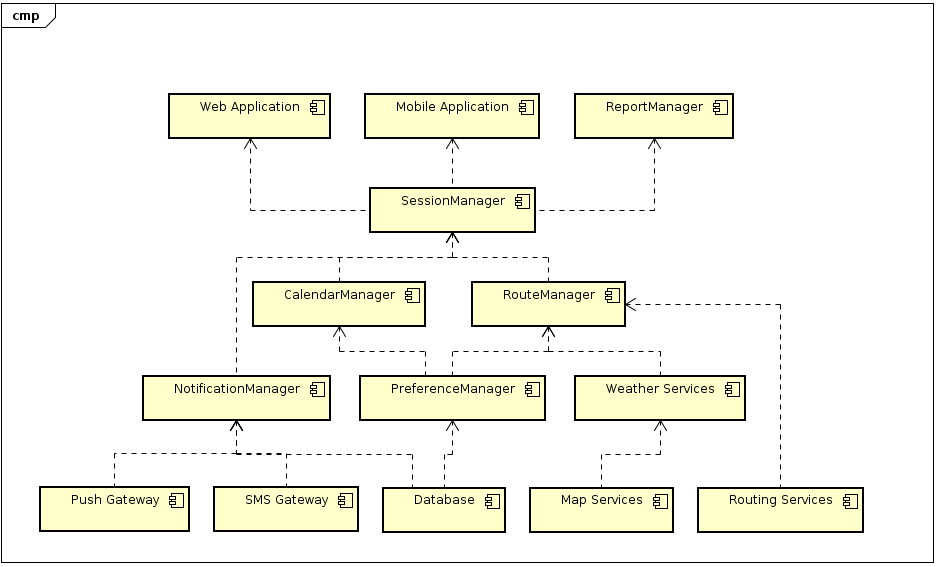
\includegraphics{Images/IntegrationDiagram.png}
	\caption{\label{fig:integration} Bottom-Up integration and testing components diagram. }
\end{sidewaysfigure}

\clearpage %Fix pictures position before this and newpage command

\subsubsection{Test Strategy}
\label{testplan}

While the system is suppose to be developed mainly through a bottom-up strategy, testing would be performed on each component as soon it is developed. Furthermore, it will also be verified the integration among component and all his dependency through specific integration tests. 

For some functionalities it is suggested to make exception because, for these ones, it is possible:

\begin{itemize}
	\item to split the deployment effort required by larger components, increasing atomicity of architecture unit in subcomponents;
	\item to anticipate the verification of some core features, that the system provides to user, far before the system test;
	\item to parallelize the development of an otherwise monolithic part of the implementation plan (particularly The \textit{SessionManager} module)
\end{itemize}

Functionalities should be verified as soon as needed components are available (list of goals and involved components is provide in \textit{Requirement Traceability} section \ref{sect:traceability}).